\section{Critical Mod}

\subsection{Concept and Critical Aim}

\textit{Trial of the Goddess} turns one of Hytale's mysterious statues
from decorative worldbuilding into the starting point of a playable ritual.
The player can pray at the statue,
receive a quest to travel \textit{Beyond the Veil},
retrieve the \textit{Sacred Flower},
and return it to the Goddess.
To survive the trial,
the player receives the \textit{Blade of Balance}.

The critical idea of the mod is that this gift is also a curse.
The Blade of Balance can defeat enemies almost instantly,
but while it is equipped,
the player is reduced to one hit point.
It also only has three empowered hits before it has to recharge.
This means that the player is extremely powerful,
but never safe.

The mod therefore changes two central expectations.
First,
a statue is no longer only atmospheric scenery,
but an object with agency,
lore,
and mechanical consequences.
Second,
combat power no longer means security.
Large monsters can become easy targets,
while small enemies such as rats become dangerous because one mistake is fatal.
The player becomes both hunter and prey at the same time.

In this way,
\textit{Trial of the Goddess} does not simply make Hytale harder.
It questions the usual relationship between power,
safety,
and mastery in combat-heavy games.

%---------------------------------------------------------------------------------------------------

\subsection{Gameplay Loop}

The gameplay loop begins when the player approaches the Goddess statue
and presses the interaction key F.
The statue is no longer passive scenery,
but becomes the starting point of the trial.
After a short dialogue sequence,
the player can either accept the Blade of Balance
or refuse the Goddess' offer.

\begin{center}
    \begin{minipage}{0.48\textwidth}
        \centering
        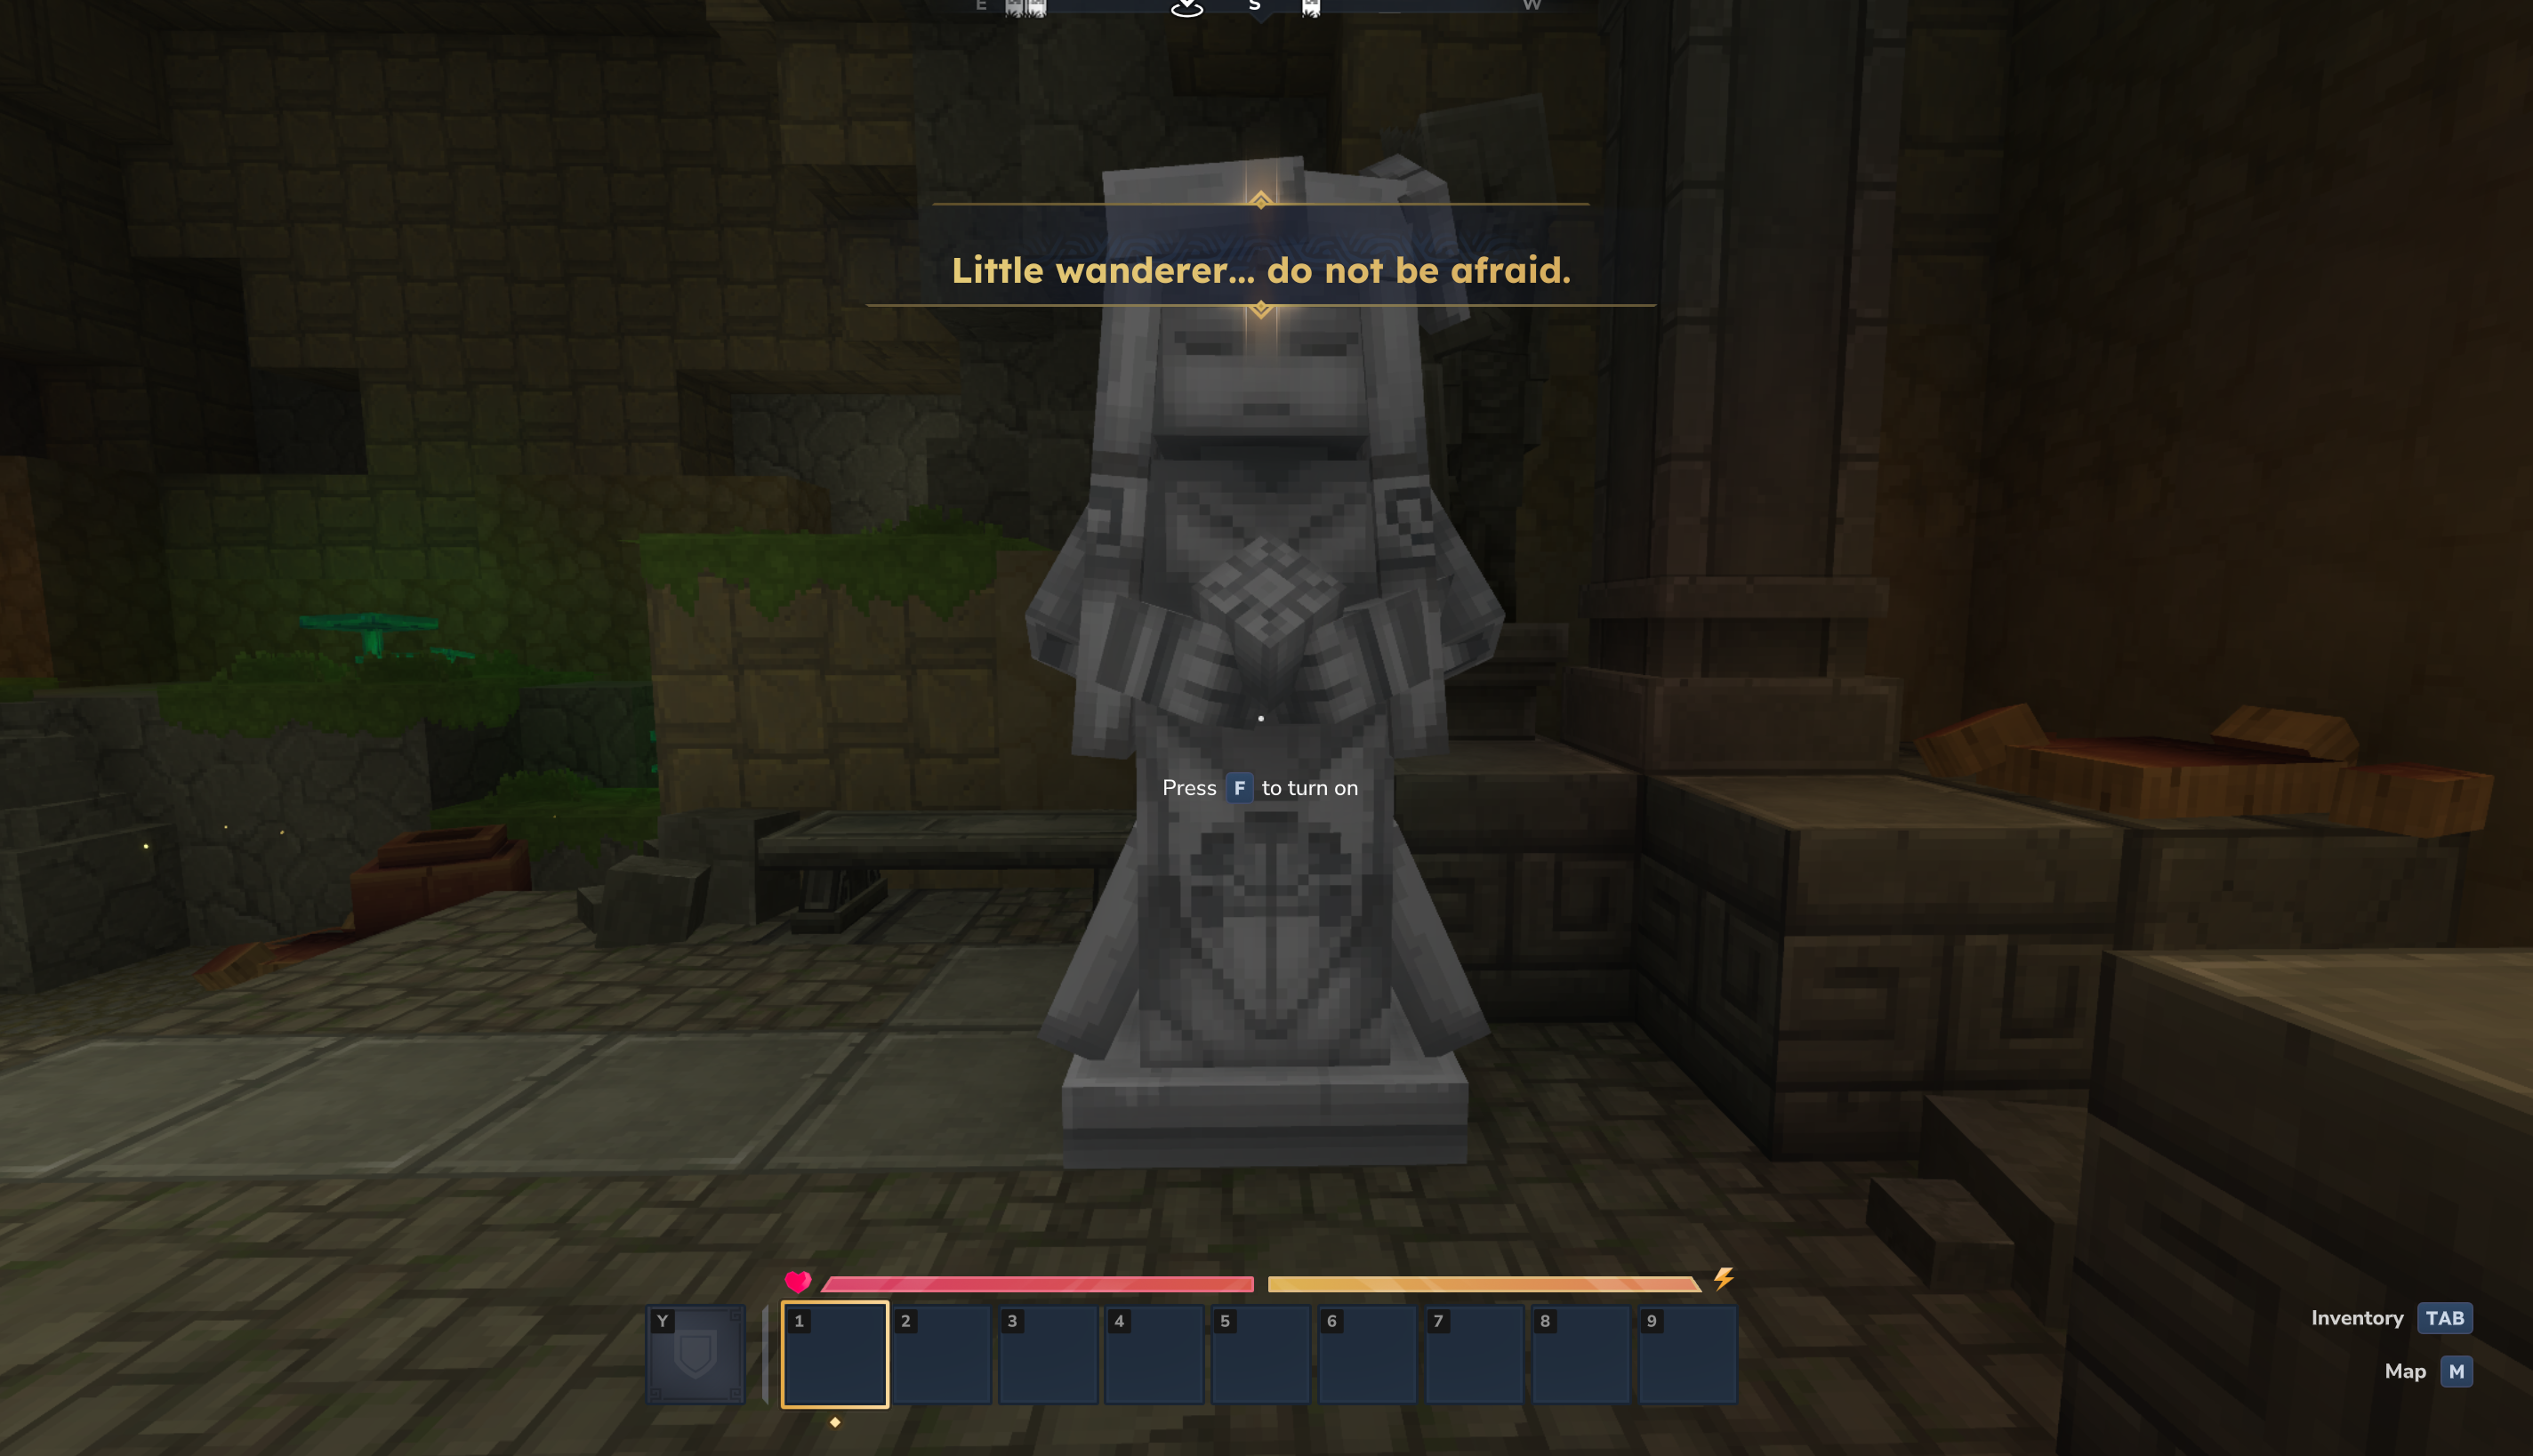
\includegraphics[width=\linewidth]{images/img_2}

        \small
        Figure: The Goddess statue functions as the starting point of the trial.
    \end{minipage}
    \hfill
    \begin{minipage}{0.48\textwidth}
        \centering
        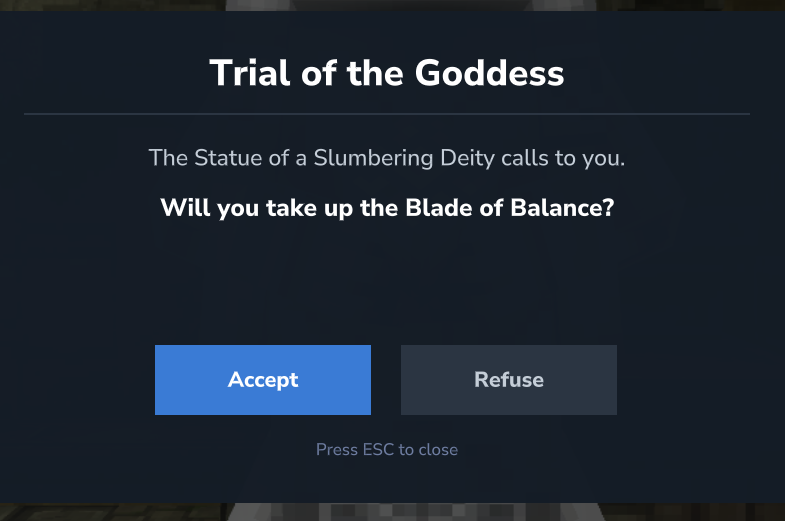
\includegraphics[width=\linewidth]{images/img_3}

        \small
        Figure: UI to accept or deny the quest.
    \end{minipage}
\end{center}

If the player accepts,
the trial starts immediately:
the Sacred Flower appears,
the player receives the Blade of Balance,
custom sound effects play,
and a wave of monsters spawns nearby.
While holding the Blade,
the player is reduced to one hit point.
The weapon can defeat enemies almost instantly,
but only has three empowered hits
before it needs to recharge for five seconds.

\begin{center}
    \begin{minipage}{0.38\textwidth}
        \centering
        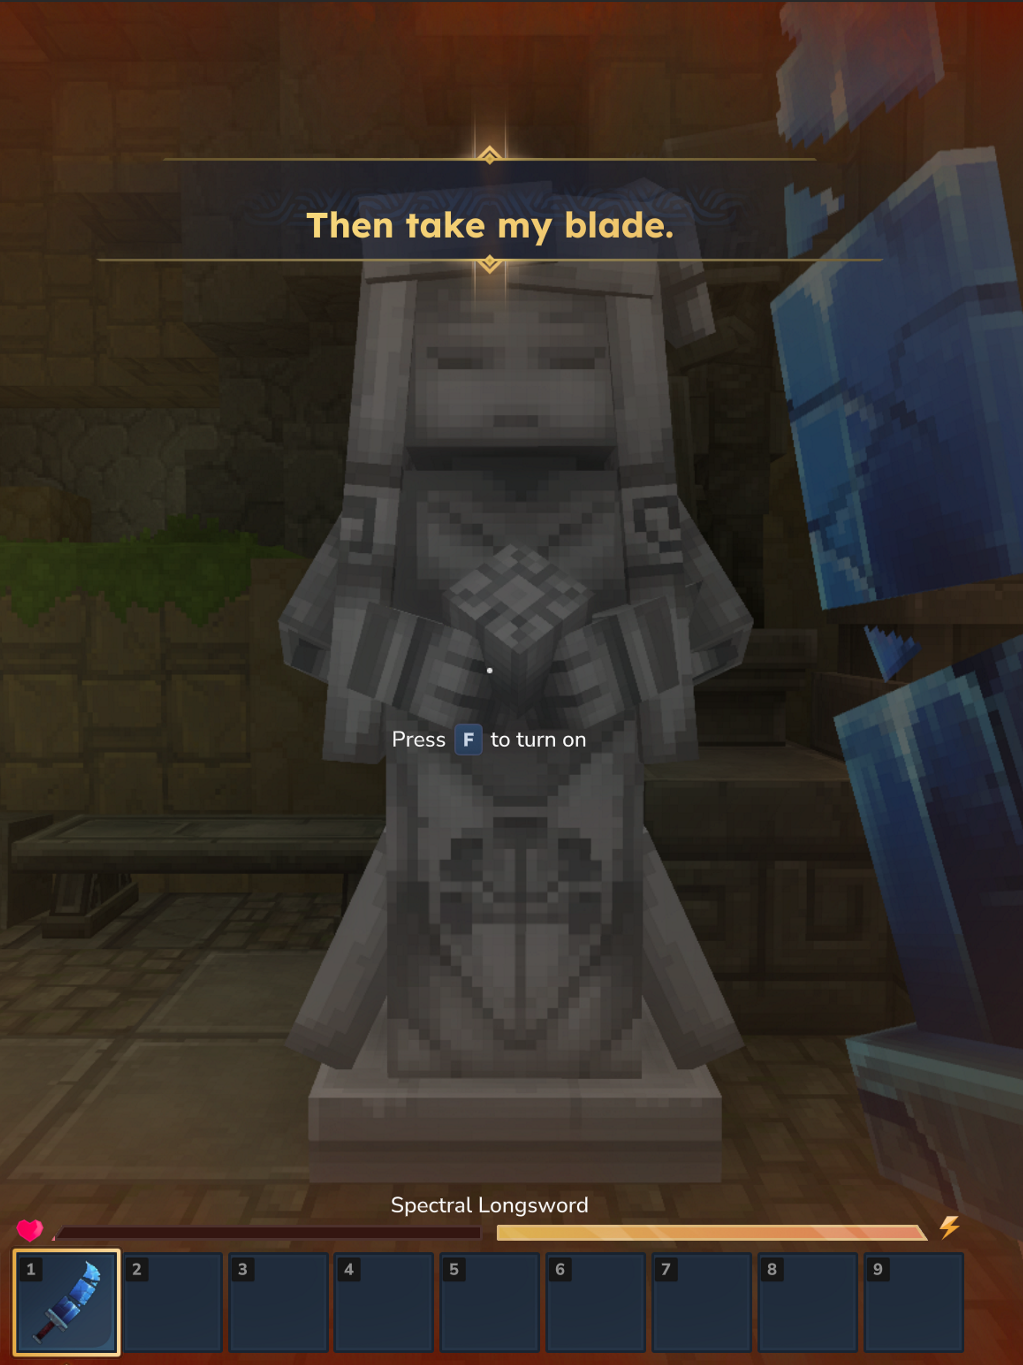
\includegraphics[width=\linewidth]{images/img_4}

        \small
        Figure: The Goddess grants the player the Blade of Balance.
    \end{minipage}
    \hfill
    \begin{minipage}{0.58\textwidth}
        \centering
        \includegraphics[width=\linewidth]{images/img_5}

        \vspace{0.4em}

        
\includegraphics[width=0.75\linewidth]{images/img_6}

        \small
        Figure: Monsters spawn nearby and the player's health is reduced
        to 1 HP while holding the Blade.
    \end{minipage}
\end{center}

\begin{center}
    \includegraphics[width=0.9\textwidth]{images/img_7}

    \small
    Figure: The Blade of Balance is empty and needs to recharge,
    while enemies continue to chase the player.
\end{center}

The objective is to find the Sacred Flower,
pick it up,
and return to the statue alive.
The flower is marked by its purple glow,
so it can be found through the environment rather than through a compass marker.

\begin{center}
    \includegraphics[width=0.75\textwidth]{images/img_8}

    \small
    Figure: The Sacred Flower is marked by its purple glow
    and can be picked up with the interaction key.
\end{center}

If the player returns without the Sacred Flower,
the Goddess reminds them that the flower is still missing.
If the player dies,
the trial fails and temporary trial items are removed.
If the player returns successfully,
the Goddess accepts the flower,
the completion dialogue plays,
and the trial is finished permanently.
As a reward,
the player keeps the Blade of Balance.

\begin{center}
    \begin{minipage}{0.49\textwidth}
        \centering
        \includegraphics[width=\linewidth]{images/img_9}

        \small
        Figure: The player returns to the statue
        while carrying the Sacred Flower.
    \end{minipage}
    \hfill
    \begin{minipage}{0.49\textwidth}
        \centering
        \includegraphics[width=\linewidth]{images/img_10}

        \small
        Figure: After the ritual is completed,
        the Goddess leaves the Blade of Balance behind as a reward.
    \end{minipage}
\end{center}

The loop can therefore be summarized as:
pray,
accept,
retrieve,
return.
Death resets the trial;
success completes it permanently.

%-----------------------------------------------------------------------------------------------------
\subsubsection{Gameplay Video}

There is a common saying that an image can speak a thousand words.
Following that logic,
a video can show a thousand images,
or around thirty images per second.
For \textit{Trial of the Goddess},
this matters because the mod depends heavily on timing,
movement,
sound,
and pressure.

Screenshots document individual moments,
but the gameplay video shows how those moments connect.
It shows the ritual as it is actually experienced:
not as separate systems,
but as one continuous sequence.
At this point,
the video can speak for itself.

\begin{center}
    \href{https://youtu.be/CctIfYMitXA?si=-ceZpl9l_rW2kv8R}
    {\textit{Trial of the Goddess} gameplay video}
\end{center}
% --------------------------------------------------------------------------------------------
\subsection{Atmosphere, Lore, and Player Experience}

The trial is designed to feel tense despite its simple structure.
The player receives a divine weapon,
but the interface constantly signals danger:
one hit point,
red screen edges,
the low-health warning,
and the blinking sound effect.
This changes combat immediately.
Large monsters can be easier to strike because they are slow and visible,
while small enemies,
especially rats,
become dangerous because they are fast,
hard to control,
and deadly during the Blade's recharge.

The atmosphere is built around contradiction.
The Goddess statue appears peaceful,
and the Goddess speaks gently,
calling the player
``little wanderer''
and telling them not to be afraid.
Yet the Blade of Balance sounds tense and threatening when it is received.
The statue feels sacred,
but the gift feels dangerous.
This makes the player question what kind of Goddess she is
and why balance requires such a violent weapon.

The lore supports this uncertainty.
The Goddess is not a normal quest giver,
but a fading deity whose name has almost disappeared.
The Sacred Flower is the last piece of herself,
so returning it is not just an objective,
but an act of restoration.
The first interaction therefore reads like a short ritual
rather than a standard quest prompt:

\begin{tcolorbox}[
    title={First statue interaction},
    colback=gray!5,
    colframe=gray!60,
    arc=2mm,
    boxrule=0.5pt
]
    \textit{You place your hand upon the cold stone.
    For a moment, nothing happens.
    Then warmth spreads through your fingers.
    Not fire.
    Not sunlight.
    Something older.}

    \medskip

    \textit{A voice unfolds inside your mind.}

    \medskip

    Little wanderer... do not be afraid.

    I am only what remains of an old goddess.

    My name has faded with the prayers of this world.

    My soul is trapped beyond the veil.

    I have accepted that I will disappear.

    But I cannot leave this world incomplete.

    Beyond the veil lies the Sacred Flower.

    It is the last piece of myself.

    Bring it to me, and I may finally slumber whole.

    Take my weapon, and cross the veil.
\end{tcolorbox}

The dialogue suggests a larger mythology
without fully explaining it:
a world where divine beings can fade,
where memory has power,
and where balance demands a cost.

My goal was to make the world feel larger than the mod itself.
Even though no additional Goddess quests are implemented yet,
the statue,
the Blade,
and the Sacred Flower should feel like fragments of something bigger.
The player should want to ask what lies beyond the veil,
why the Goddess needs the flower,
and whether other statues might hide similar stories.


Writing the dialogue was also a design problem.
Hytale's title display worked best with one short line at a time,
so the text had to be split into ritual-like fragments.
After testing,
I added a skip feature:
pressing the interaction key again while the Goddess is speaking
opens the offer page immediately.
This keeps the atmosphere for the first interaction,
but avoids making repeated attempts feel slow.

Additional dialogue variants,
including refusal,
returning without the Sacred Flower,
and completing the trial,
are included in Appendix~\ref{app:dialogue}.

% --------------------------------------------------------------------------------------------
\subsection{Implementation Overview}

Although \textit{Trial of the Goddess} feels like one continuous ritual,
the implementation is split into several smaller systems.
This separation was necessary because the mod changes many parts of the game at once:
statue interaction,
dialogue,
UI,
trial state,
the Blade's health and damage behavior,
flower spawning,
monster spawning,
persistence,
and cleanup.

The most important design decision was to separate the trial state from the visible effects.
The core state decides what is allowed:
whether the trial has not started,
has been offered,
is active,
has failed,
or has already been completed.
Other systems then react to that state by showing dialogue,
granting the Blade,
spawning enemies,
placing the Sacred Flower,
or cleaning up temporary objects.
This prevented different parts of the mod from contradicting each other.

\begin{center}
    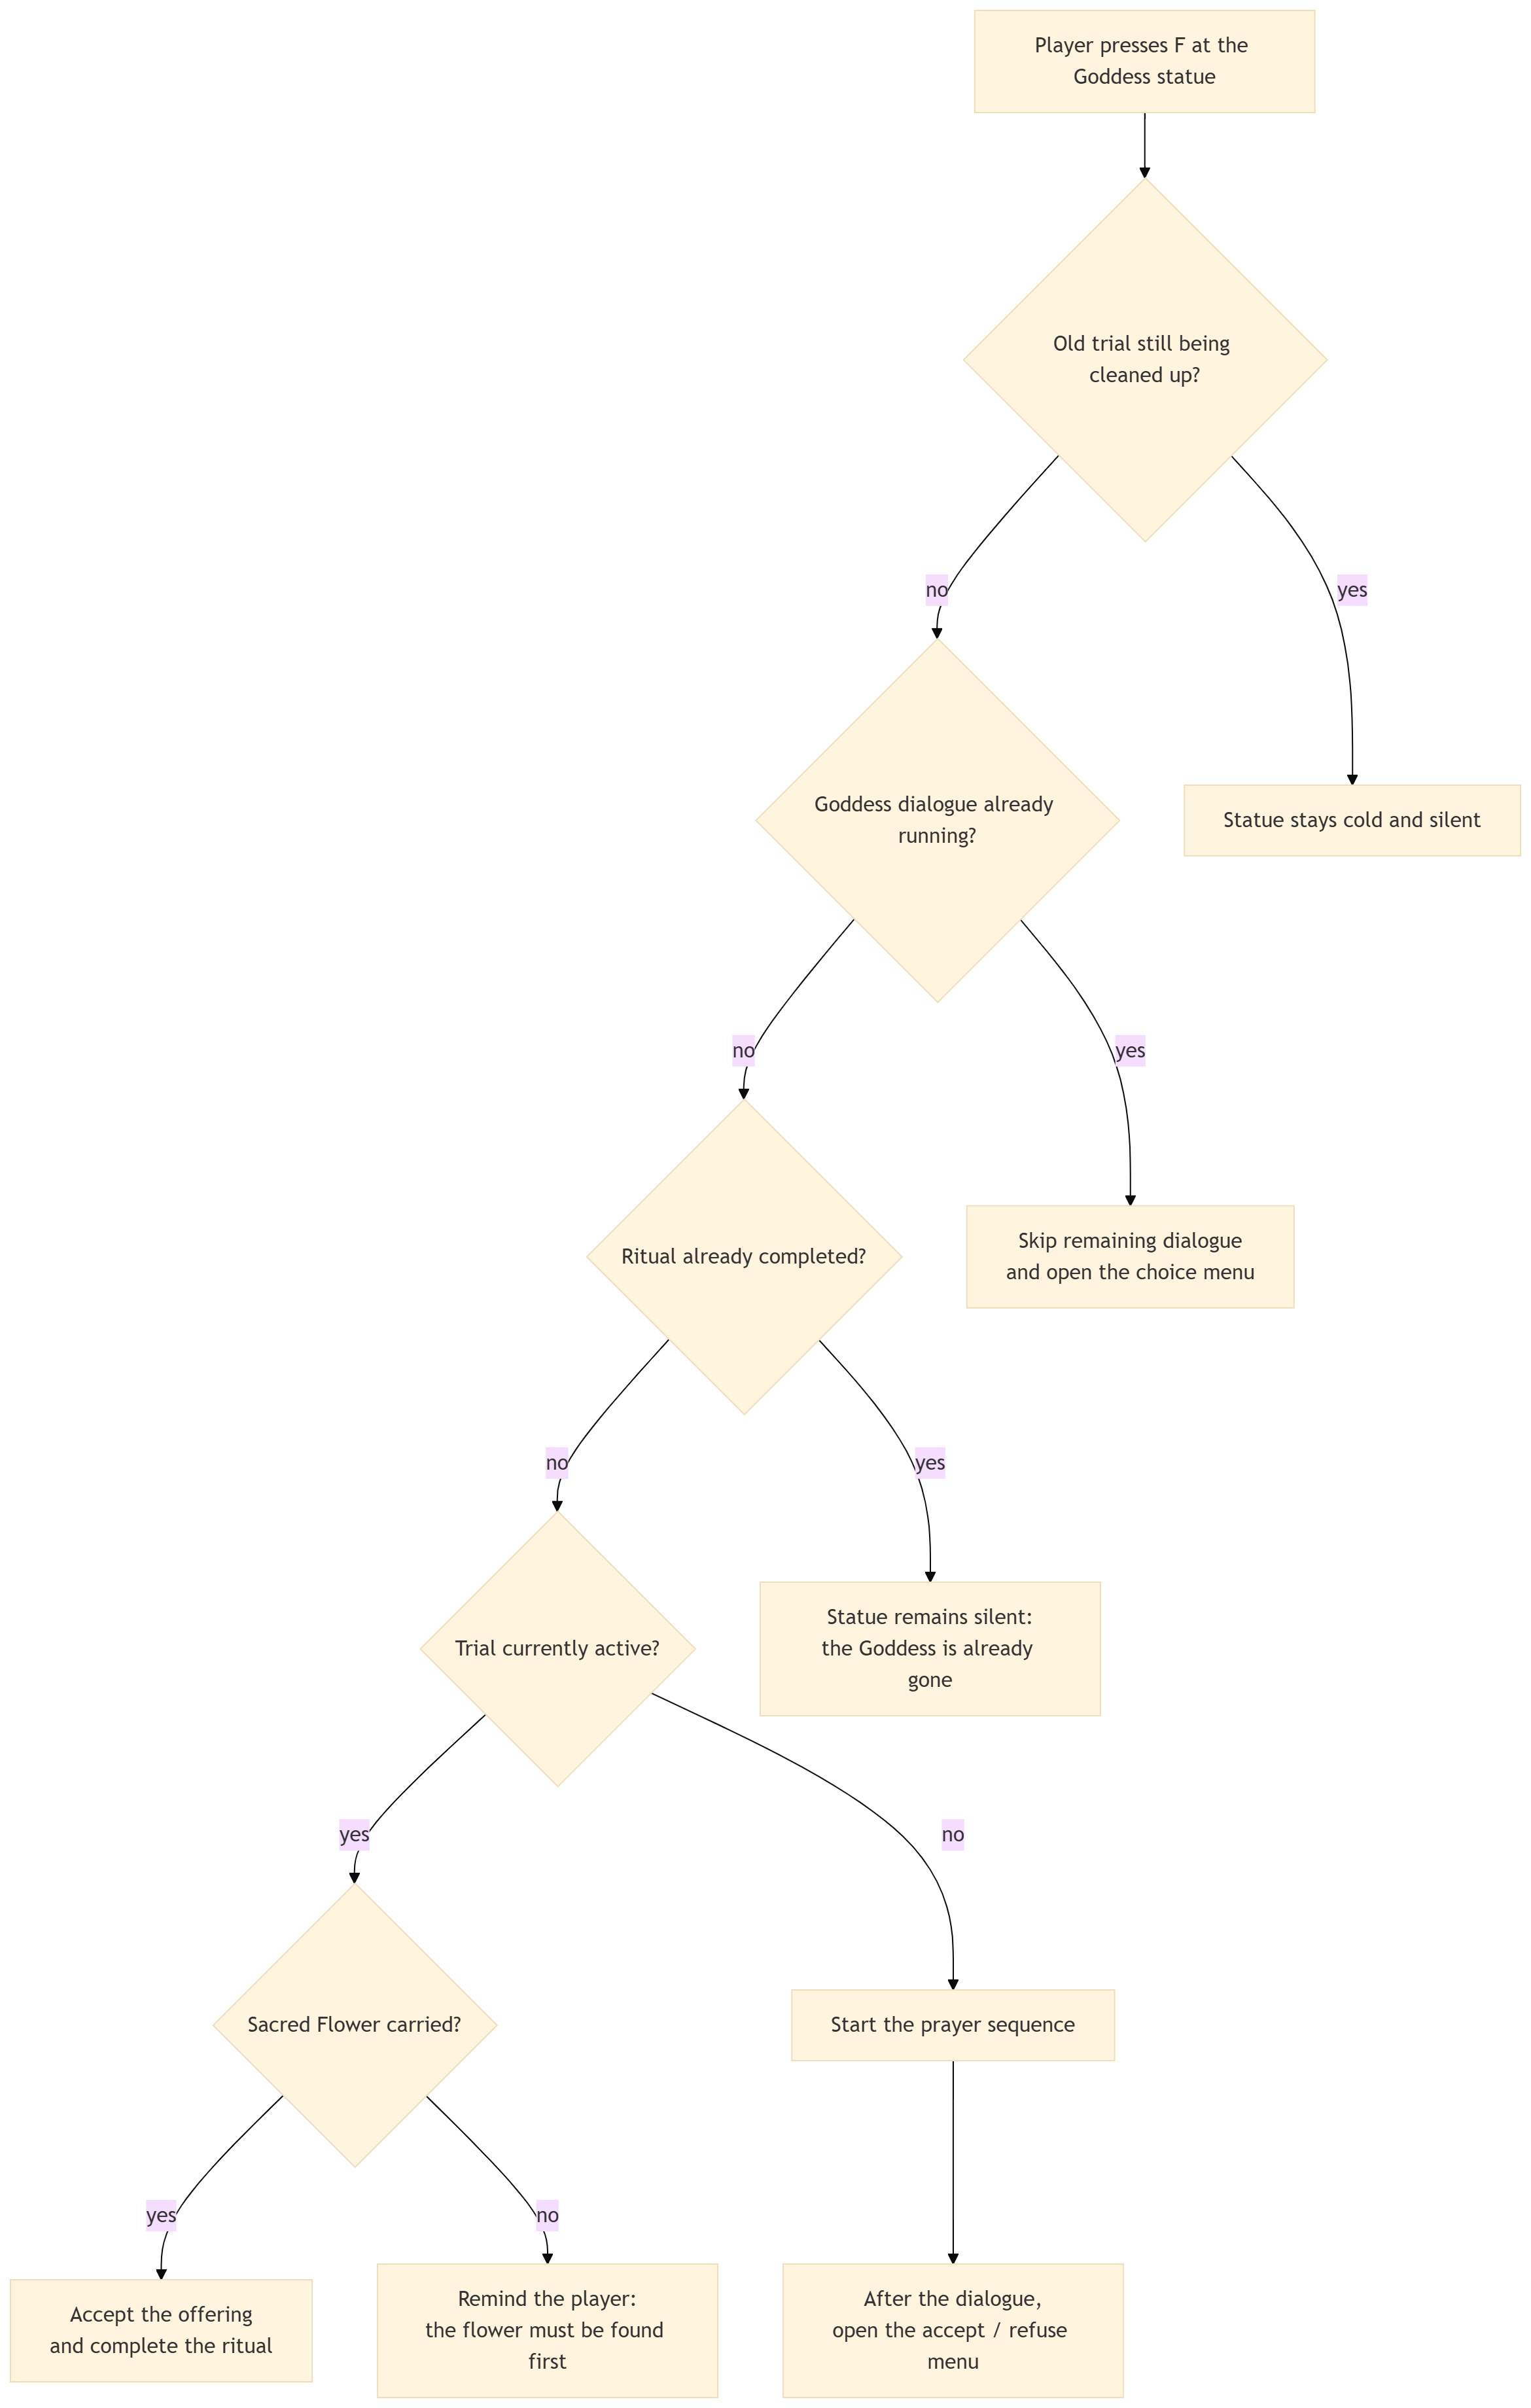
\includegraphics[height=0.55\textheight,keepaspectratio]{images/statuelogic}

    \small
    Figure: State-dependent behavior of the Goddess statue.
    The same interaction can start the prayer sequence,
    skip dialogue,
    remind the player,
    complete the ritual,
    or stay silent depending on the current trial state.
\end{center}

The Blade of Balance is handled as its own gameplay system.
It does not simply increase damage.
While the Blade is held,
the player's current health is forced back to one hit point,
and the empowered attacks are limited by a recharge cycle.
This keeps the critical idea of the mod inside the code structure:
power is granted,
but it is never safe.

\begin{center}
    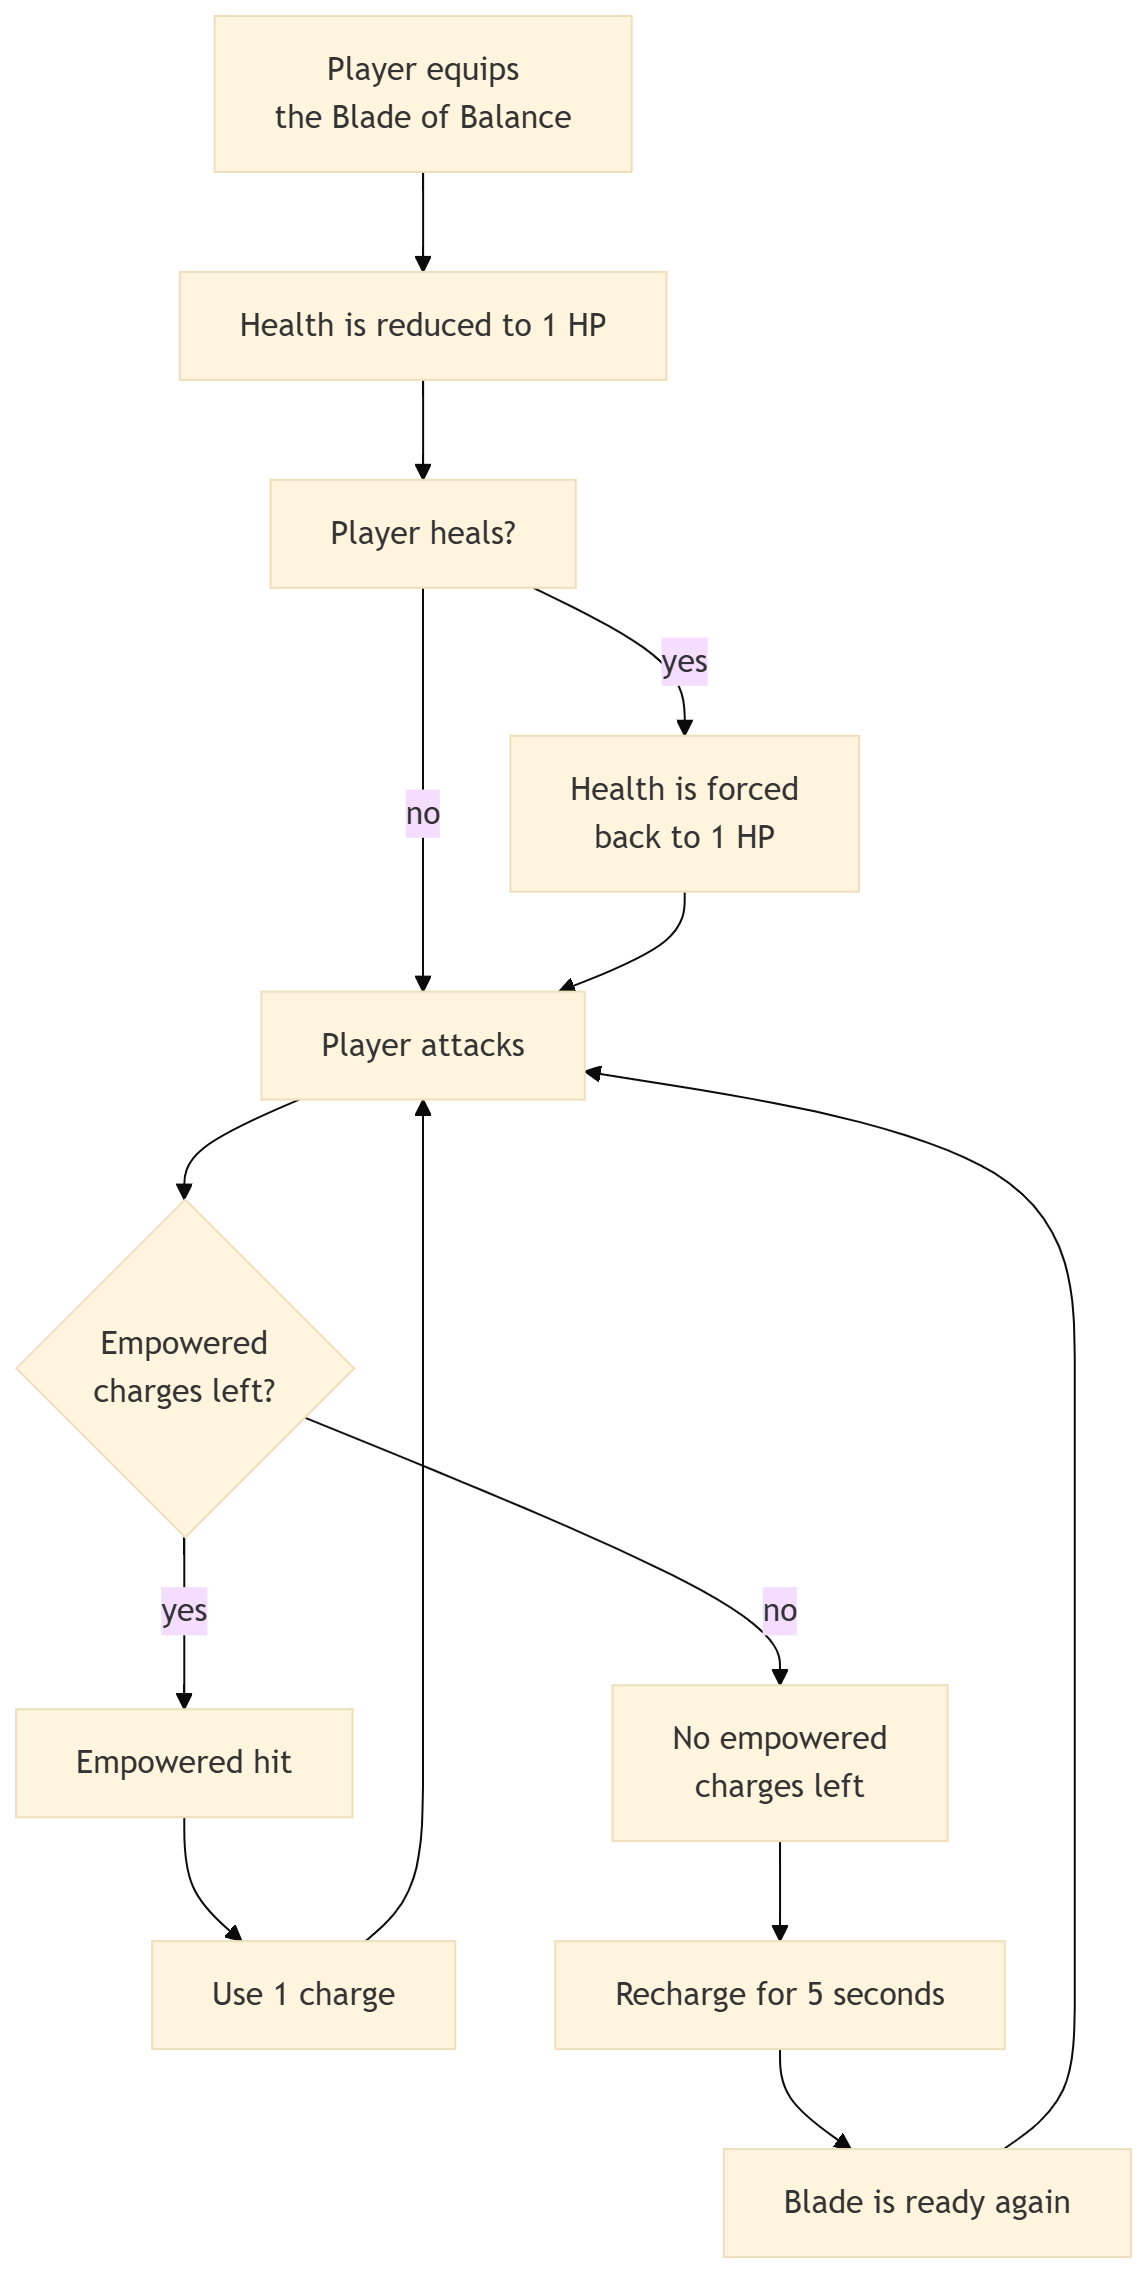
\includegraphics[height=0.55\textheight,keepaspectratio]{images/swordlogic}

    \small
    Figure: Logic of the Blade of Balance.
    While the blade is held during or after the trial,
    the player is kept at 1 HP.
    Its empowered attacks can only be used a limited number of times
    before a recharge phase begins.
\end{center}

The main technical struggles came from the limits of Hytale's current toolkit.
The statue only became interactive after its JSON asset configuration pointed
to the custom \texttt{GoddessTrial\_Statue} interaction,
so asset files became part of the logic rather than only visuals.
The Sacred Flower could not reliably spawn through a fully dynamic terrain search,
so I used manually configured positions in a fixed world.
A compass marker was replaced by the flower's purple glow,
and recurring monster reinforcements were disabled after they caused
entity-store problems.

These compromises shaped the final mod.
Where Hytale's intended systems worked,
I used them directly:
custom interactions,
UI pages,
sound events,
item effects,
and block JSON files.
Where they became unreliable,
I changed the design instead of forcing the original plan.
Detailed architecture diagrams,
asset configuration notes,
and the full implementation breakdown are included in
Appendix~\ref{app:implementation-details}.

The source code of the mod is available in the GitHub repository:

\begin{center}
    \href{https://github.com/ayanomaliy/GoddessTrial.git}
    {\textit{Trial of the Goddess} GitHub repository}
\end{center}

% --------------------------------------------------------------------------------------------
\subsection{Custom Sound and Zelda Inspiration}

The atmosphere of \textit{Trial of the Goddess} is inspired by shrine
and goddess interactions in
\textit{The Legend of Zelda: Breath of the Wild}
and
\textit{Tears of the Kingdom}.
I used these games as references for ancient voices,
ritual interaction,
sacred spaces,
and reward-through-trial,
without copying their audio directly.

Because of this,
I recreated the intended sound myself in Serum instead of reusing copyrighted material.
This mattered because the mod was not only a programming task:
it also required asset creation,
sound design,
and decisions about how the final experience should feel.

\begin{center}
    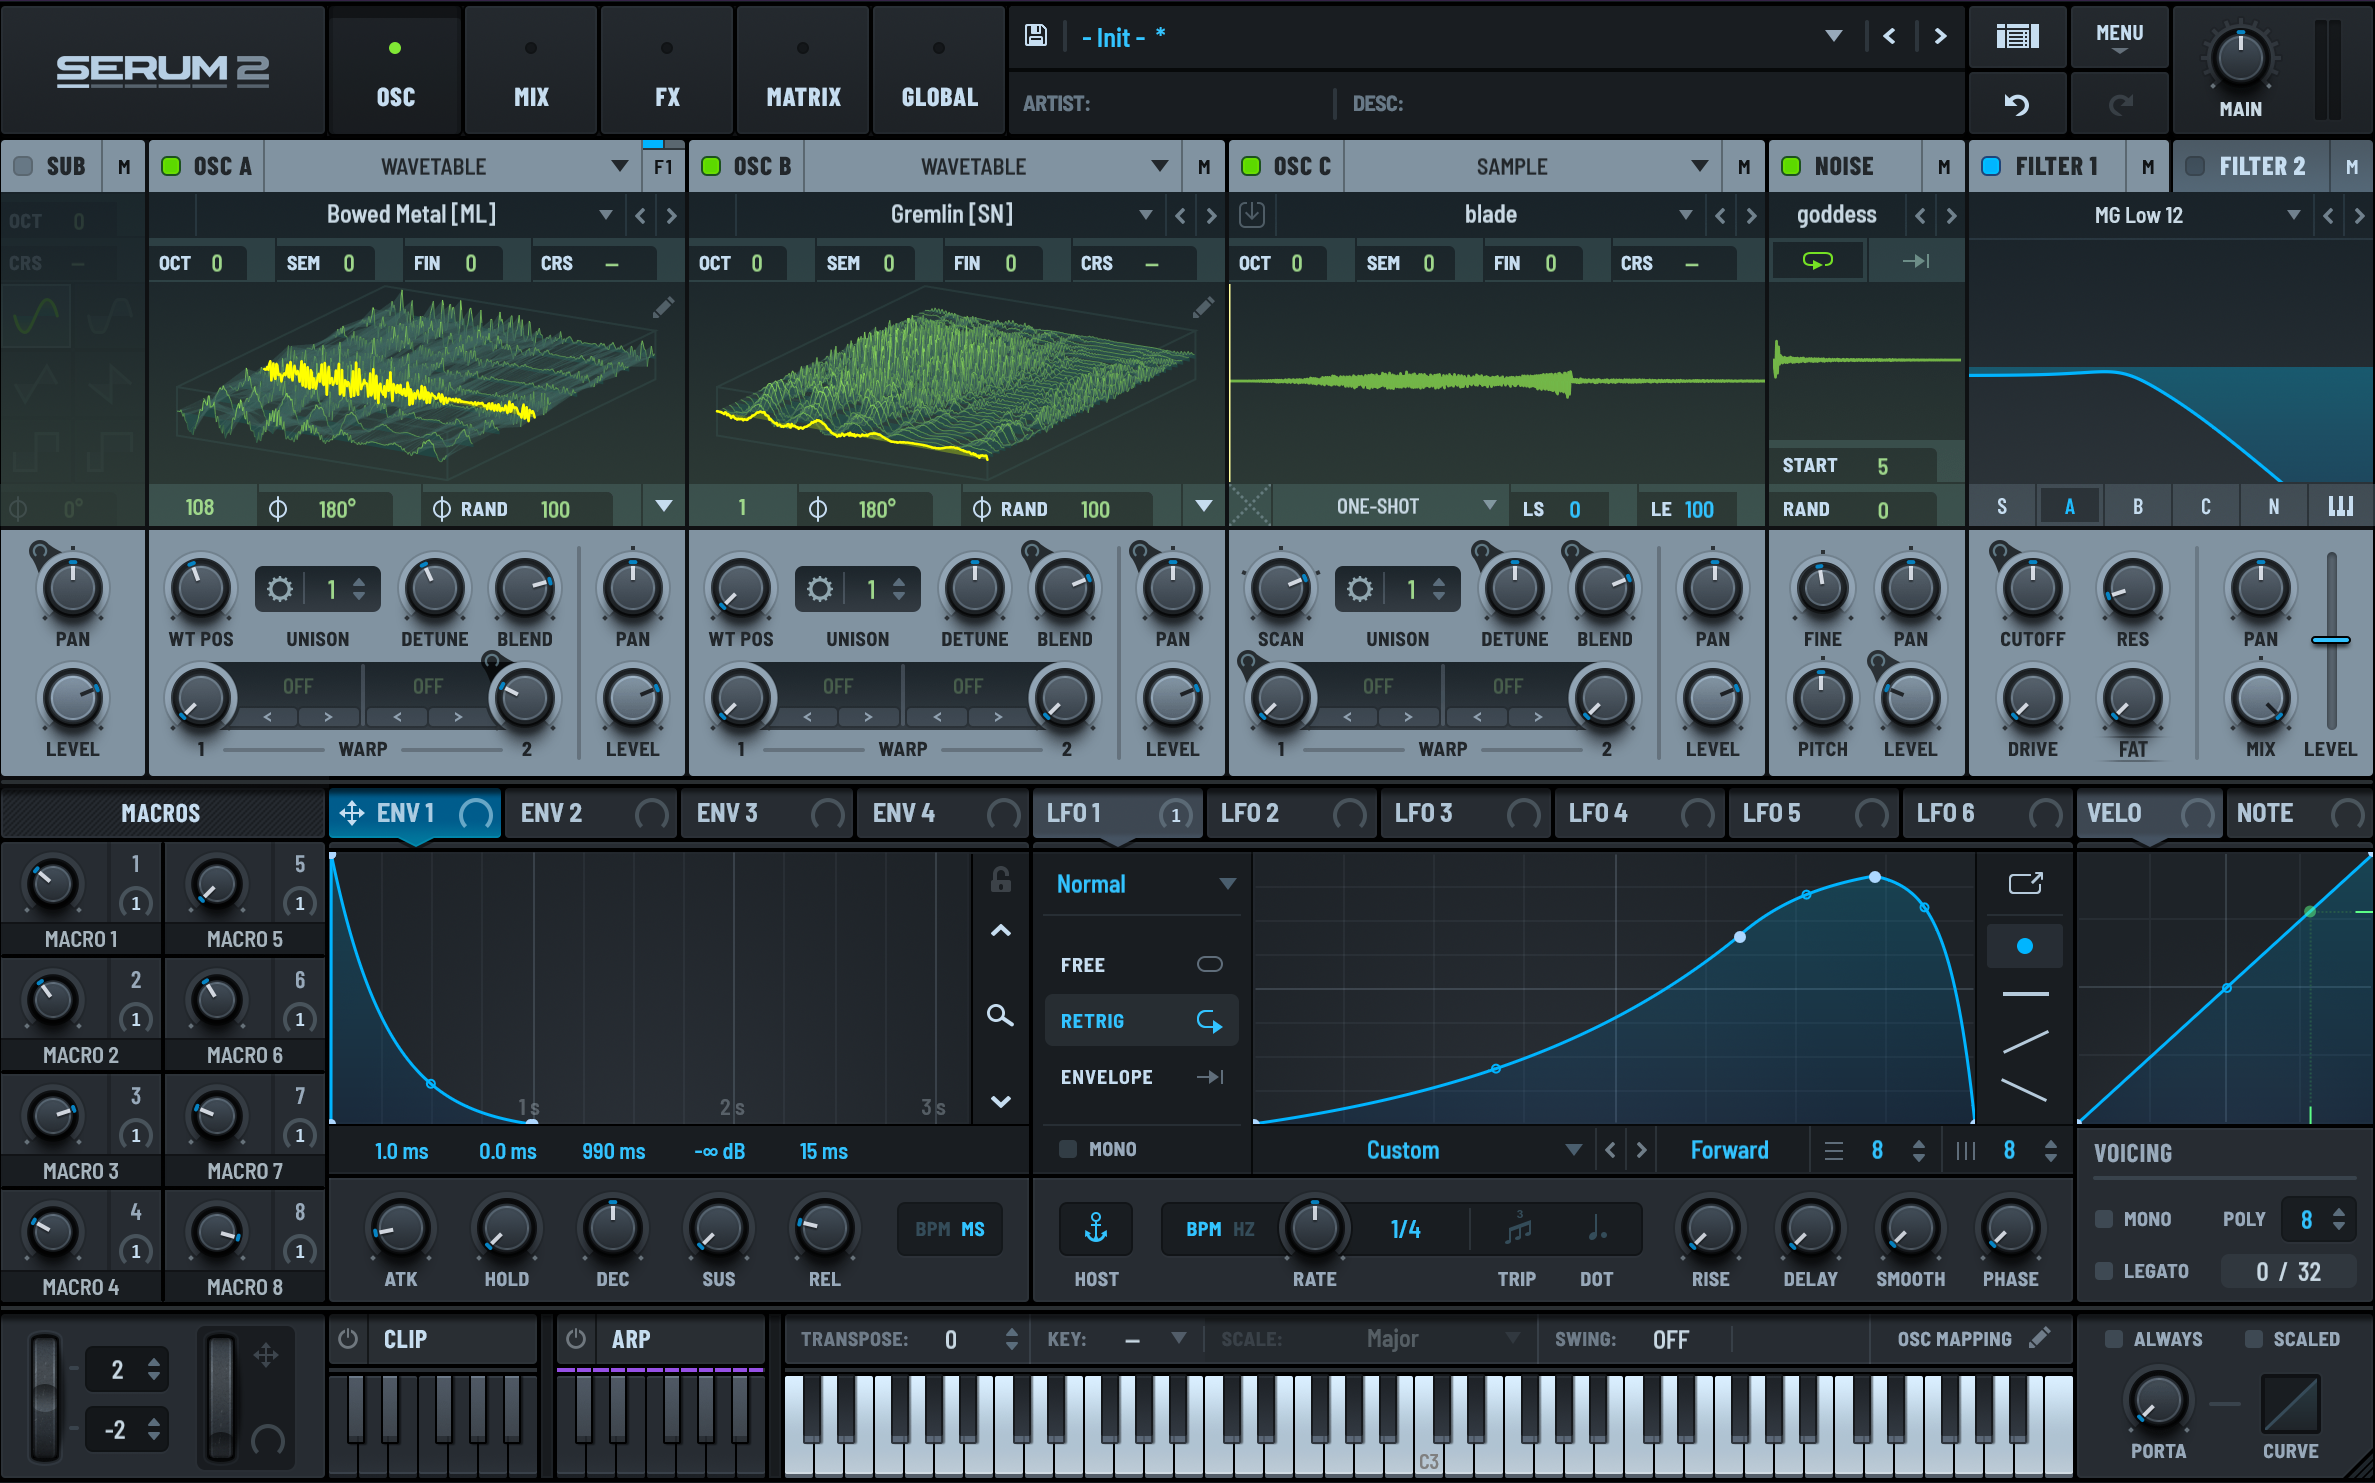
\includegraphics[width=0.65\textwidth]{images/img_11}

    \small
    Figure: Creating custom sound effects for the mod in Serum.
\end{center}